\documentclass[10pt]{scrartcl}
\usepackage{amsmath,amsthm,amssymb,mathtools,xfrac}
\usepackage{enumerate}
\usepackage[utf8]{inputenc}
%\usepackage{german}
\usepackage{a4wide}
\usepackage{graphics}
\usepackage{graphicx}
\usepackage[T1]{fontenc}
\usepackage{epsfig}
\usepackage{libertine}
\usepackage[pdftex]{hyperref}
\usepackage{refcount}
\usepackage{framed} 
\usepackage{xcolor}
\usepackage{multicol}
\usepackage{enumitem}
\usepackage{caption}
\usepackage{gensymb}
\usepackage[export]{adjustbox}

\topmargin-.5in \textheight9in \oddsidemargin0in \textwidth6.5in

\begin{document}


\begin{minipage}{.5\textwidth}
{\scshape Department of Mathematics and Informatics \\
University of Cologne\\}
\small Prof. Dr. Gregor Gassner \\
\small Dr. Andrés Rueda-Ramírez \\
\end{minipage}
\hfill
\begin{minipage}{.3\textwidth}
\begin{flushright}

\includegraphics[width=3cm]{figs/logo-uni-koeln.jpg}\\
\today
\end{flushright}
\end{minipage}

\begin{center}
{\Large\bfseries
An Introduction to Climate Modeling}\\
\vspace{0.2cm}
{\bfseries Milestone 4 - The pointwise zero-dimensional Energy Balance Model}
\end{center}



\section{The pointwise zero-dimensional Energy Balance Model}
 In the previous milestone you have implemented the zero-dimensional EBM for the global mean temperature. In this milestone you will use this model to compute the mean temperature for the northern and southern hemisphere. Furthermore you will implement the EBM model pointwise for each grid point.

\begin{enumerate}
\item[1.]Implement the functions \small\texttt{\detokenize{calc_mean_north}} \normalsize and \small\texttt{\detokenize{calc_mean_south}} \normalsize analogous to the function \small\texttt{\detokenize{calc_mean}} \normalsize from milestone 3 to calculate the mean value on the southern and northern hemisphere of a given parameter for an input matrix of values of that paramer in each grid point.

\item[2.]Use the \small\texttt{\detokenize{calc_equilibrium}} \normalsize function from milestone 3 to compute the EBM for the northern and southern hemisphere by substituting the \small\texttt{\detokenize{calc_mean}} \normalsize function with the two functions from task 1. What differences do you notice to the mean temperature result from milestone 3?

\item[3.]Now use the \small\texttt{\detokenize{calc_equilibrium}} \normalsize function to compute the EBM for each grid point by looping over every grid point and substituting the mean values with the values on each grid point. Plot the results as an animation similar to milestone 2.

\item[4.]Use the results of the pointwise calculation in task 3 to calculate the mean temperatures over the whole globe, the northern hemisphere and the southern hemisphere using the functions \small\texttt{\detokenize{calc_mean}} \normalsize, \small\texttt{\detokenize{calc_mean_north}} \normalsize and \small\texttt{\detokenize{calc_mean_south}} \normalsize. What differences are there to the results of the EBM calculations that are based on the mean values from the start?

\item[5.] What is the temperature in Cologne according to the pointwise EBM? Compare it to the other results. What is noticeable?

\end{enumerate}

\newpage

\section{Control Solutions}

\begin{figure}[!htb]
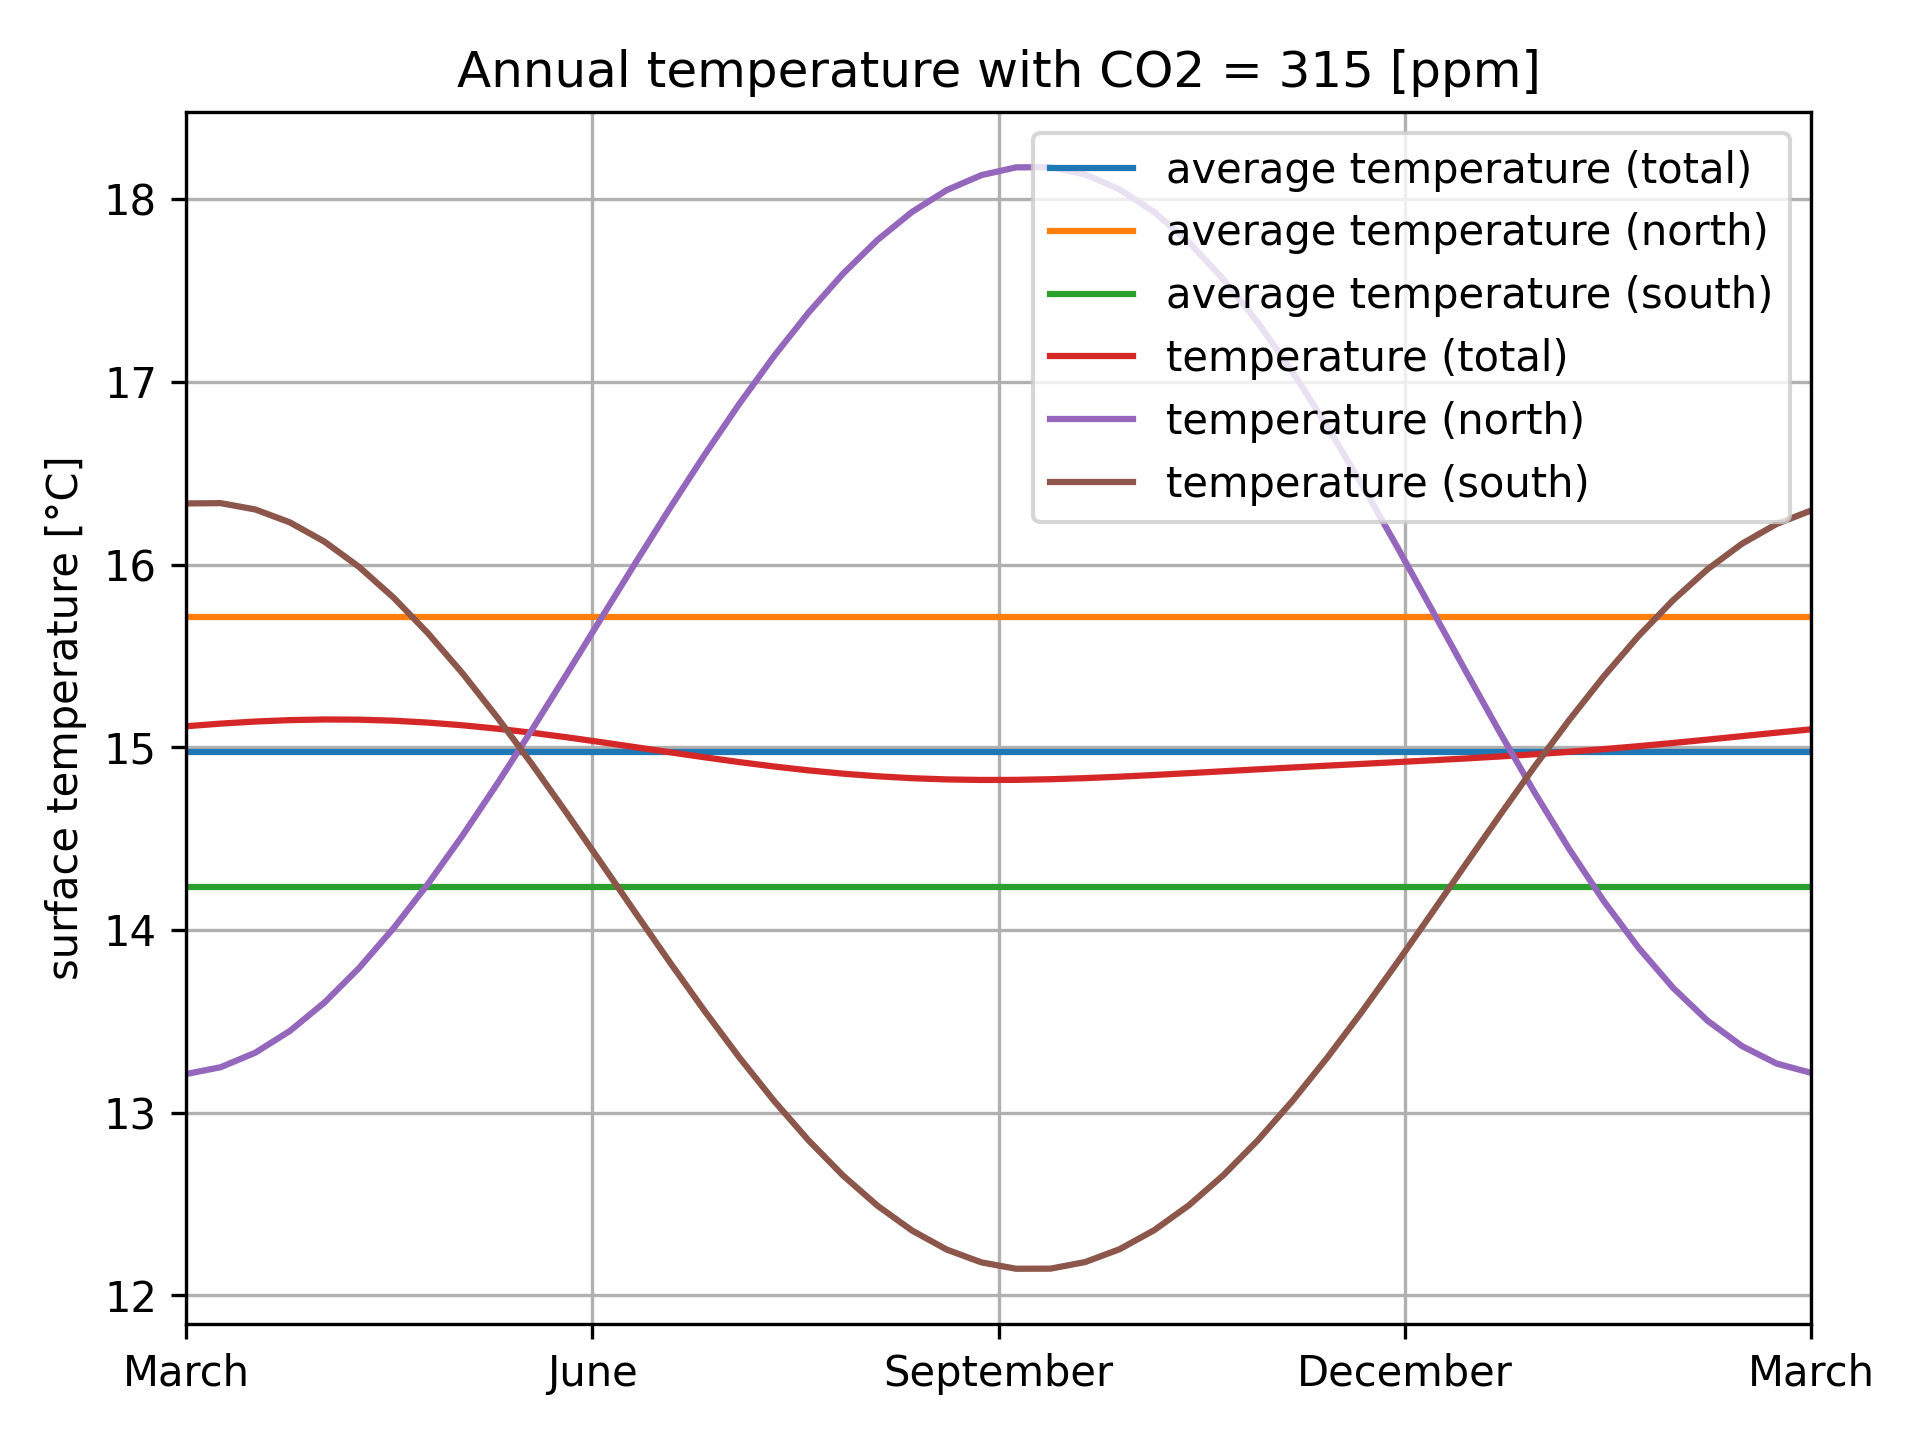
\includegraphics[width=0.6\linewidth,center]{figs/mean_temperatures.png}
\caption{EBM results for the mean temperatures}
\end{figure}

\begin{figure}[!htb]
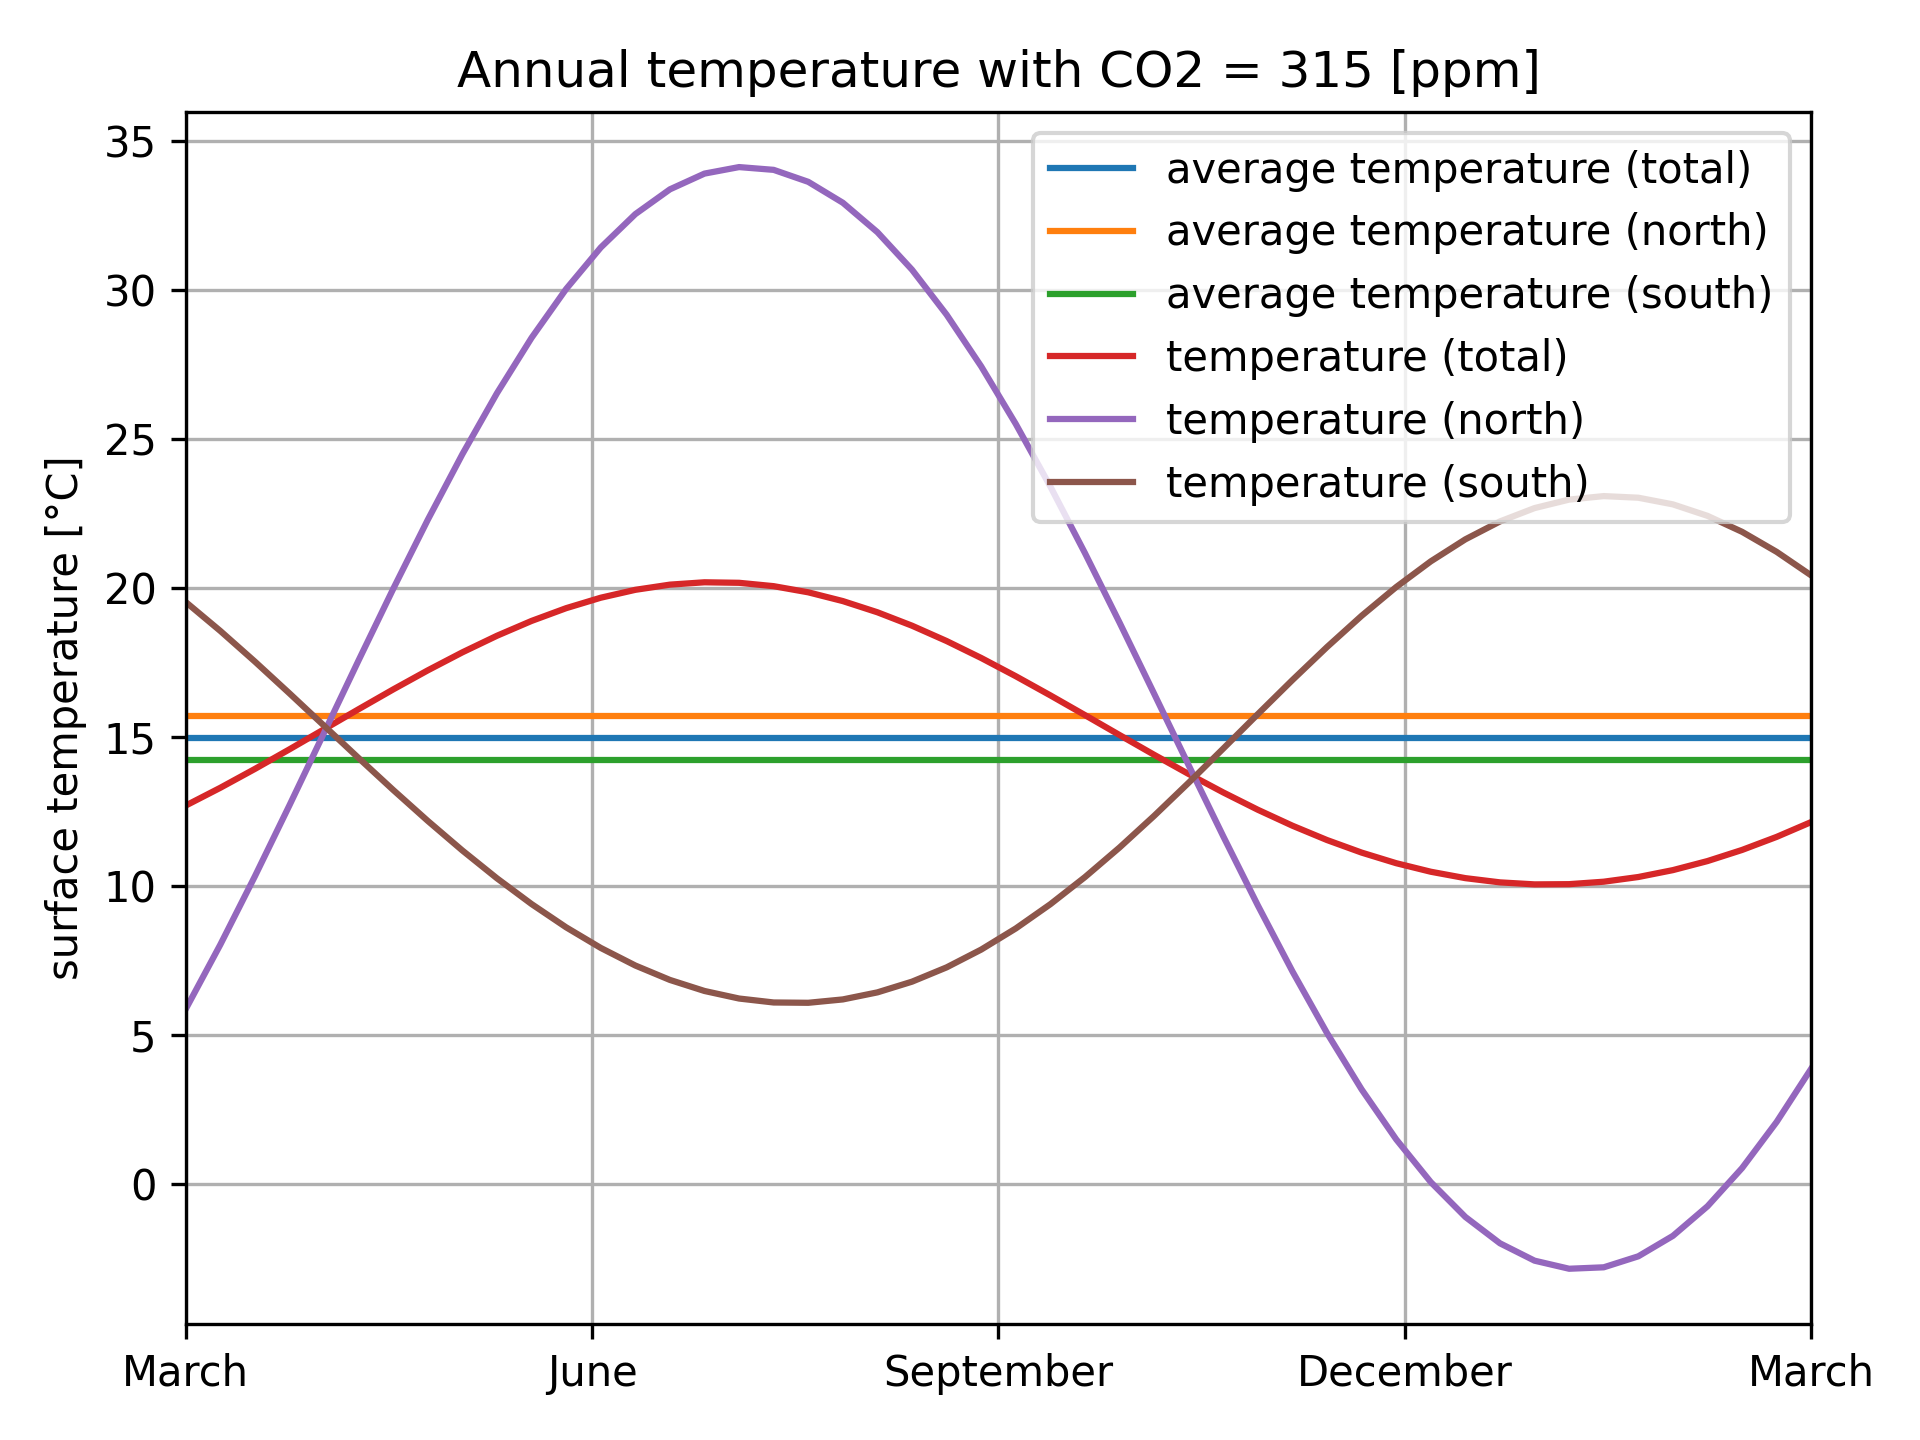
\includegraphics[width=0.6\linewidth,center]{figs/mean_temperatures_pointwise.png}
\caption{EBM results for the mean temperature based on the pointwise calculations}
\end{figure}

\begin{figure}[!htb]
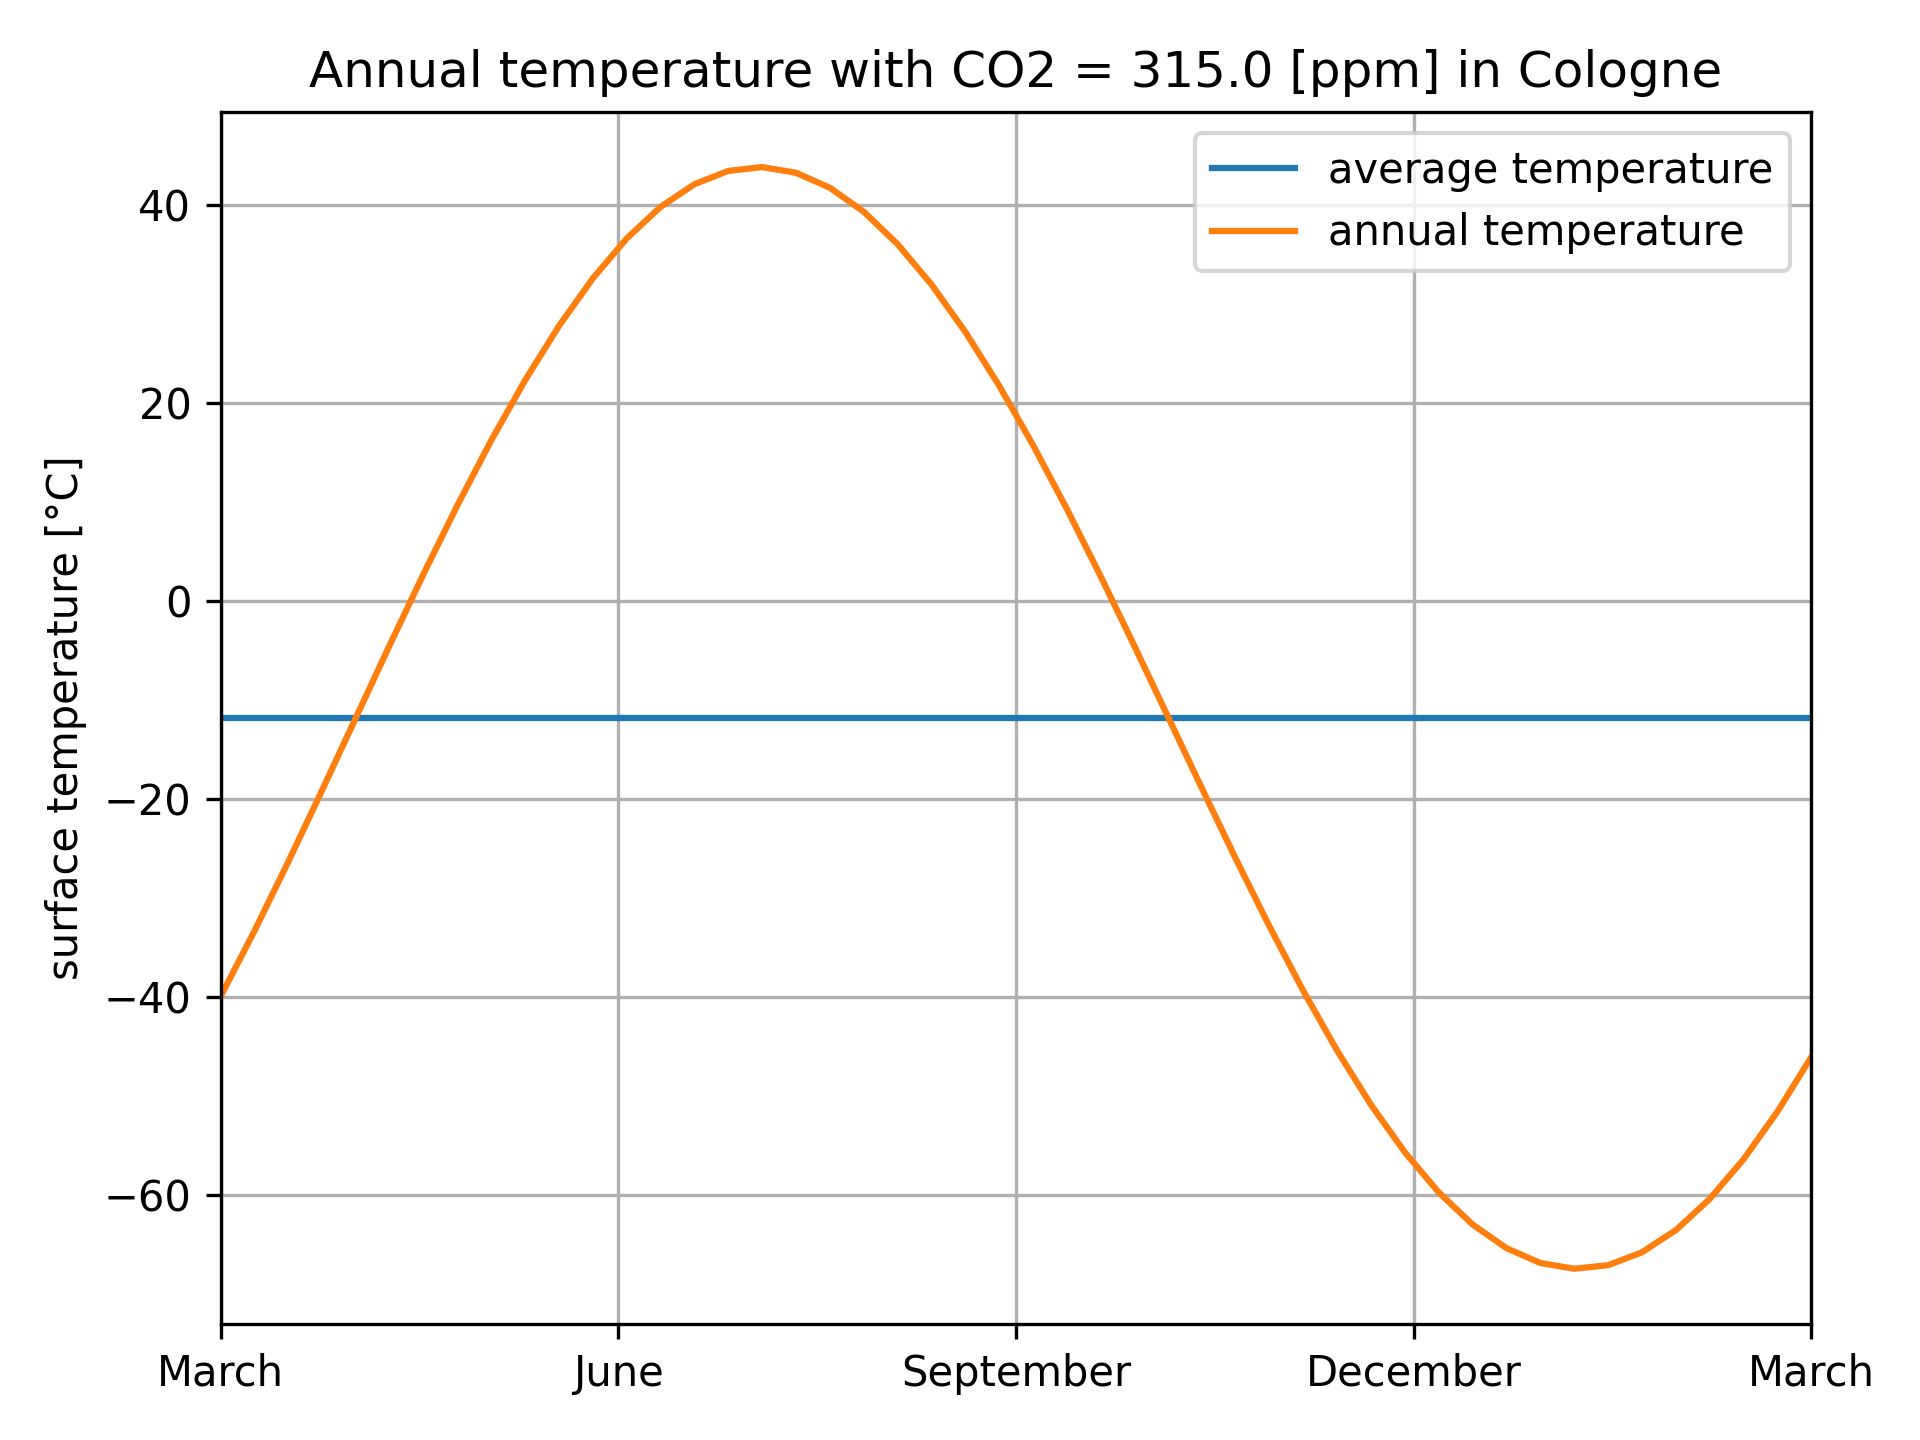
\includegraphics[width=0.6\linewidth,center]{figs/temperature_cologne.png}
\caption{pointwise EBM results}
\end{figure}

\begin{figure}[!htb]
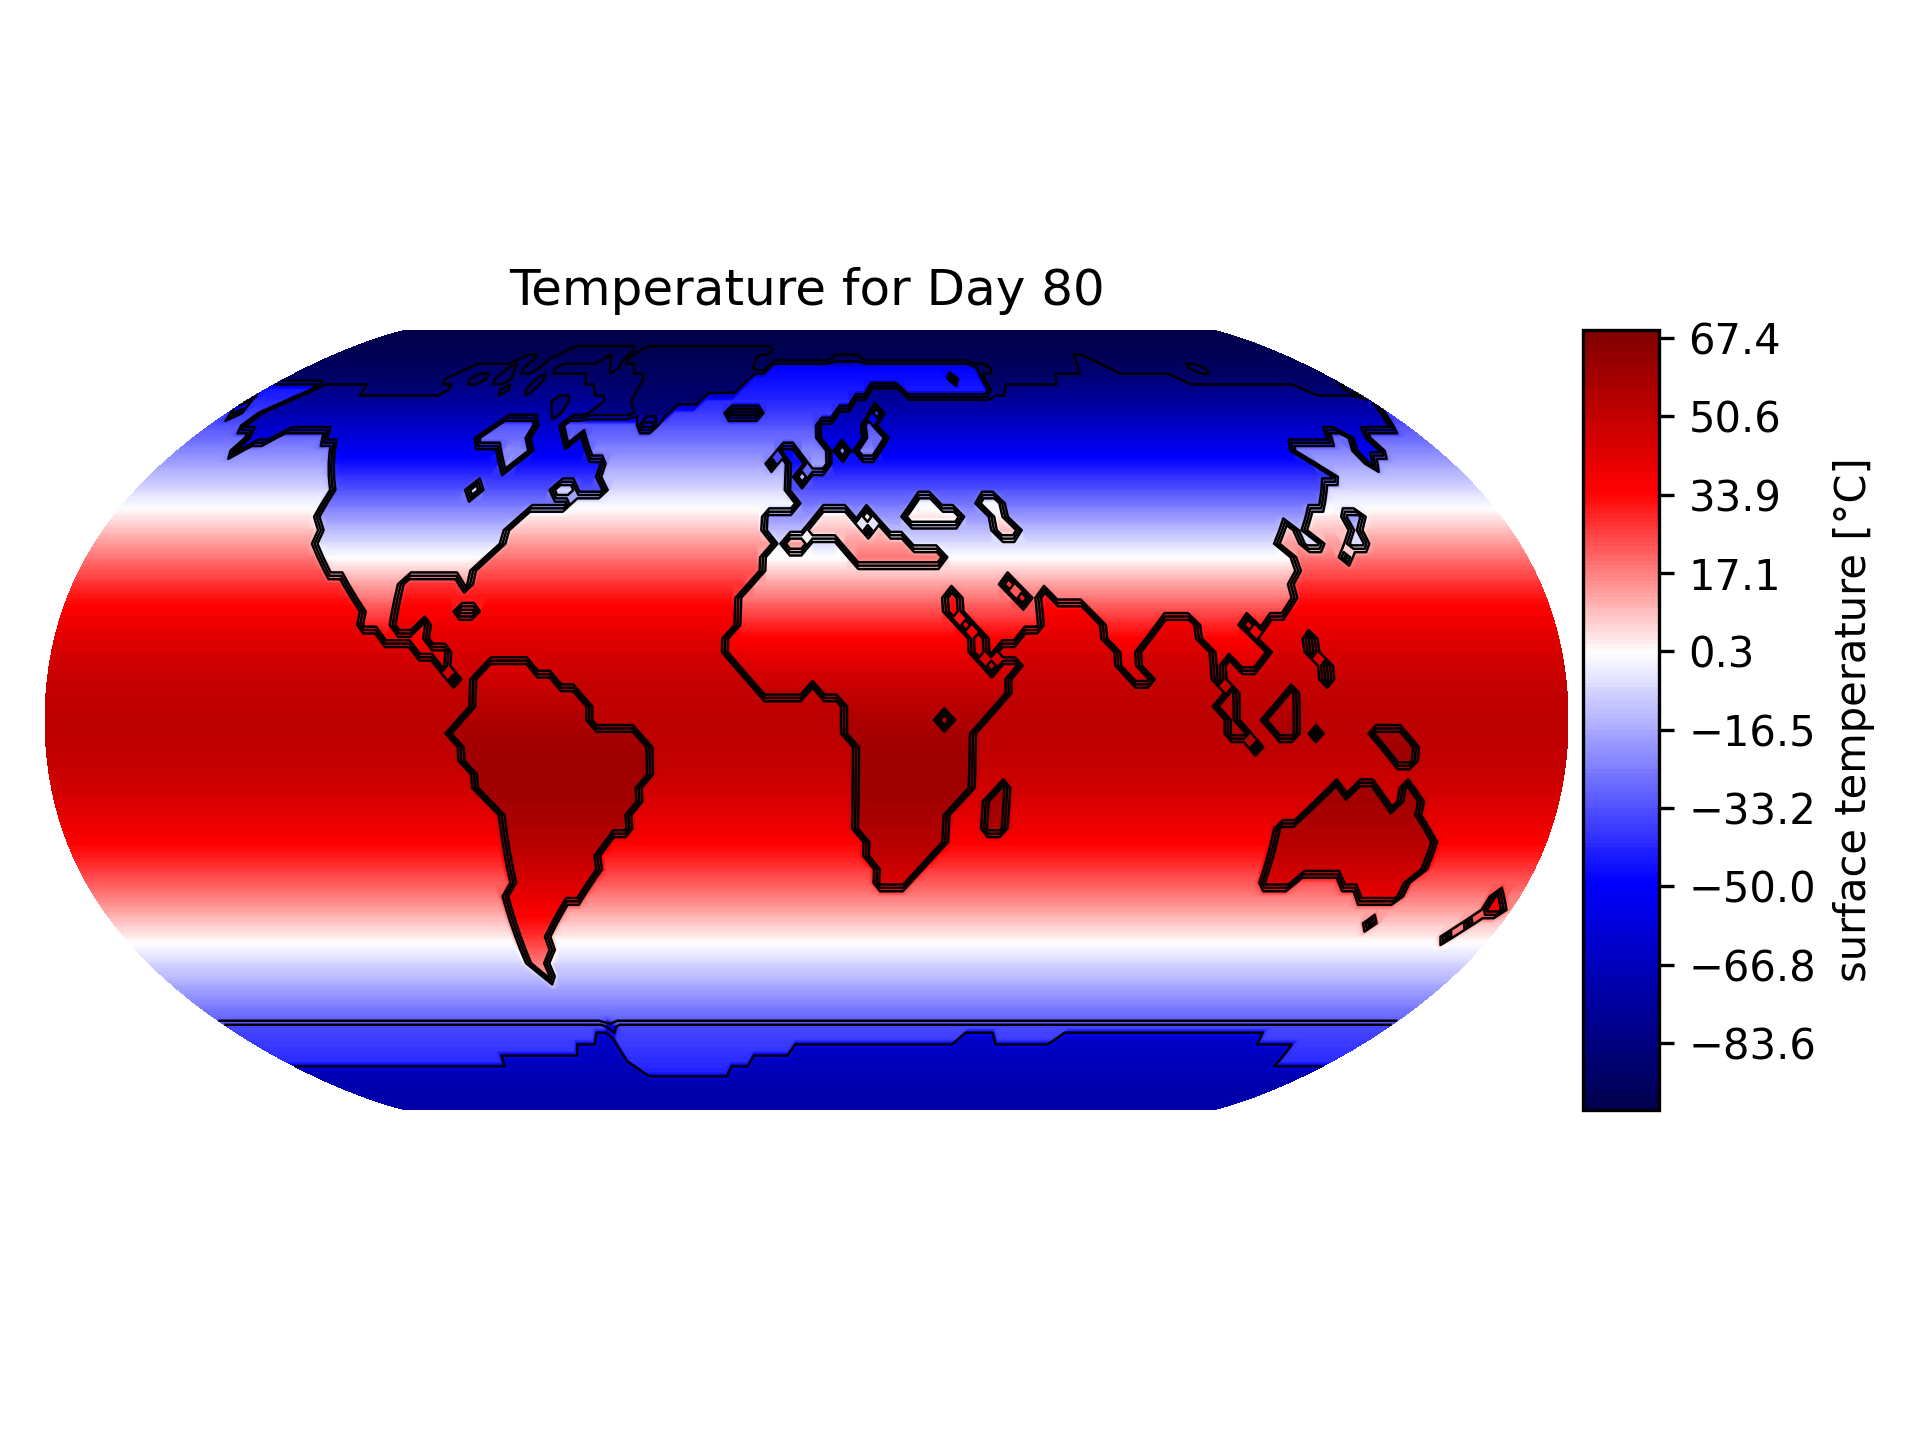
\includegraphics[width=0.7\linewidth,center]{figs/annual_temperature_day_80.png}
\caption{Time evolution of the temperature based on NASA data}
\end{figure}

\end{document}
